% !TEX encoding = UTF-8
% !TEX TS-program = pdflatex
% !TEX root = ../tesi.tex
% !TEX spellcheck = it-IT

%**************************************************************
\chapter{Procedure di controllo di qualità di processo}
%**************************************************************
La qualità dei processi è basato sul \textit{ciclo di Deming}. Tale modello è studiato per il miglioramento continuo della qualità in un'ottica a lungo raggio. Il \textit{ciclo di Deming} è chiamato anche \gls{pdca} a causa delle quattro fasi che lo compongono:
\begin{itemize}
	\item \textbf{Plan:} fase di pianificazione in cui vengono definite attività, risorse, scandenze e responsabilità;
	\item \textbf{Do:} fase in cui si eseguono le attività pianificate;
	\item \textbf{Check:} fase di verifica in cui si controllano i risultato ottenuti nella fase \textit{Do} e si confrontano con quelli pianificati della fase \textit{Plan};
	\item \textbf{Act:} fase in cui si mette in pratica il miglioramento continuo dei processi utilizzando i risultati della verifica per modificare gli aspetti critici dei processi in esame.
\end{itemize}

Per migliorare la qualità, le quattro fasi devono ruotare costantemente, tenendo come criterio principale la qualità di processo.

\begin{figure}[h]
\centering
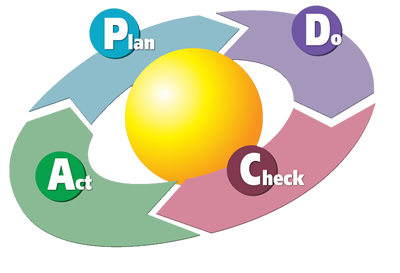
\includegraphics[width=0.6\linewidth]{immagini/pdca}
\caption[Il ciclo PDCA]{Il ciclo PDCA}
\label{fig:pdca}
\end{figure}

%\epigraph{Citazione}{Autore della citazione}



